% Created 2012-10-10 Wed 19:58
\documentclass[11pt]{article}
\usepackage[utf8]{inputenc}
\usepackage{fixltx2e}
\usepackage{url}
\usepackage{graphicx}
\usepackage{minted}
\usepackage{color}
\usepackage{longtable}
\usepackage{float}
\usepackage{wrapfig}
\usepackage{soul}
\usepackage{textcomp}
\usepackage{amsmath}
\usepackage{marvosym}
\usepackage{wasysym}
\usepackage{latexsym}
\usepackage{amssymb}
\usepackage[linktocpage,
  pdfstartview=FitH,
  colorlinks,
  linkcolor=blue,
  anchorcolor=blue,
  citecolor=blue,
  filecolor=blue,
  menucolor=blue,
  urlcolor=blue]{hyperref}
\usepackage{attachfile}
\tolerance=1000
\usepackage{adjustbox}
\usepackage{anysize}
\marginsize{1in}{1in}{1in}{1in}
\providecommand{\alert}[1]{\textbf{#1}}

\title{Molecular Simulation HOMEWORK 3}
\author{Zhongnan Xu}
\date{10/12/12 Thursday}
\hypersetup{
  pdfkeywords={},
  pdfsubject={},
  pdfcreator={Emacs Org-mode version 7.8.11}}

\begin{document}

\maketitle

\setcounter{tocdepth}{3}
\tableofcontents
\vspace*{1cm}


\section{Reaction energy of CO oxidation}
\label{sec-1}
\subsection{Compute the reaction energy for CO + 1/2 O$_{2}$ $\rightarrow$ CO$_{2}$}
\label{sec-1-1}
\label{rxn-energy}

Use a cutoff energy of 250 eV. The molecules should all be relaxed to their lowest energy geometry (perform a geometry optimization). Demonstrate that all the forces on the molecule are less than 0.05 eV/\AA{}.


\begin{minted}[frame=lines,fontsize=\scriptsize,linenos]{python}
from ase import Atoms, Atom
from jasp import *
import numpy as np
np.set_printoptions(precision=3, suppress=True)

CO = Atoms([Atom('C', (0, 0, 0)),
            Atom('O', (1.2, 0, 0))],
           cell=(10, 10, 10))
O2 = Atoms([Atom('O', (0, 0, 0)),
            Atom('O', (1.23, 0, 0))],
           cell=(9.8, 9.9, 10))
CO2 = Atoms([Atom('O', (0, 0, 0)),
             Atom('C', (1.16, 0, 0)),
             Atom('O', (2.32, 0, 0))],
            cell=(10, 10, 10))
with jasp('prob1a/CO',
          xc='PBE', lreal=False,
          encut=250, prec='Accurate',
          kpts=(1, 1, 1), ismear=1, sigma=0.05,
          ibrion=1, nsw=50, ediffg=-0.05, isif=2,
          atoms=CO) as COcalc:
    try:
        eCO = CO.get_potential_energy()
        fCO = CO.get_forces()
    except:
        pass
with jasp('prob1a/O2',
          xc='PBE', lreal=False,
          encut=250, prec='Accurate',
          kpts=(1, 1, 1), ismear=1, sigma=0.05,
          ibrion=1, nsw=50, ediffg=-0.05, isif=2,
          atoms=O2) as O2calc:
    try:
        eO2 = O2.get_potential_energy()
        fO2 = O2.get_forces()
    except:
        pass
with jasp('prob1a/CO2',
          xc='PBE', lreal=False,
          encut=250, prec='Accurate',
          kpts=(1, 1, 1), ismear=1, sigma=0.05,
          ibrion=1, nsw=50, ediffg=-0.05, isif=2,
          atoms=CO2) as CO2calc:
    try:
        eCO2 = CO2.get_potential_energy()
        fCO2 = CO2.get_forces()
    except:
        pass

re = eCO2 - eCO - 0.5*eO2
print 'The total energy of CO is {0:1.3f}'.format(eCO)
print 'The forces (eV/angstrom) on the atoms in CO are'
print 'C: {0}'.format(fCO[0])
print 'O: {0}\n'.format(fCO[1])
print 'The total energy of O2 is {0:1.3f}'.format(eO2)
print 'The forces (eV/angstrom) on the atoms in O2 are'
print 'O: {0}'.format(fO2[0])
print 'O: {0}\n'.format(fO2[1])
print 'The total energy of CO2 is {0:1.3f}'.format(eCO2)
print 'The forces (eV/angstrom) on the atoms in CO2 are'
print 'O: {0}'.format(fCO2[0])
print 'C: {0}'.format(fCO2[1])
print 'O: {0}\n'.format(fCO2[2])
print 'The reaction energy is {0:1.3f}'.format(re)
\end{minted}


\begin{verbatim}
The total energy of CO is -15.168
The forces (eV/angstrom) on the atoms in CO are
C: [-0.033  0.     0.   ]
O: [ 0.033  0.     0.   ]

The total energy of O2 is -8.719
The forces (eV/angstrom) on the atoms in O2 are
O: [ 0.019  0.     0.   ]
O: [-0.019  0.     0.   ]

The total energy of CO2 is -23.508
The forces (eV/angstrom) on the atoms in CO2 are
O: [-0.015  0.     0.   ]
C: [ 0.  0.  0.]
O: [ 0.015  0.     0.   ]

The reaction energy is -3.980
\end{verbatim}
\subsection{Convergence test}
\label{sec-1-2}

Repeat the previous problem at 350, 450, and 500 eV. Reoptimize the geometry at each ENCUT value. Compare (in a graph) the convergence of the total energy of each species with the convergence of the reaction energy. Which converges faster?


\begin{minted}[frame=lines,fontsize=\scriptsize,linenos]{python}
from ase import Atoms, Atom
from jasp import *
import numpy as np
np.set_printoptions(precision=3, suppress=True)

CO = Atoms([Atom('C', (0, 0, 0)),
            Atom('O', (1.2, 0, 0))],
           cell=(10, 10, 10))
O2 = Atoms([Atom('O', (0, 0, 0)),
            Atom('O', (1.23, 0, 0))],
           cell=(9.8, 9.9, 10))
CO2 = Atoms([Atom('O', (0, 0, 0)),
             Atom('C', (1.16, 0, 0)),
             Atom('O', (2.32, 0, 0))],
            cell=(10, 10, 10))
dirs = ('/e350', '/e450', '/e500')
cuts = (350, 450, 500)
eCOs = []
eO2s = []
eCO2s = []

for d, cut in zip(dirs, cuts):
    with jasp('prob1b' + d + '/CO',
              xc='PBE', lreal=False,
              encut=cut, prec='Accurate',
              kpts=(1, 1, 1), ismear=1, sigma=0.05,
              ibrion=1, nsw=50, ediffg=-0.05, isif=2,
              atoms=CO) as COcalc:
        try:
            eCO = CO.get_potential_energy()
            eCOs.append(eCO)
        except:
            pass
    with jasp('prob1b' + d + '/O2',
              xc='PBE', lreal=False,
              encut=cut, prec='Accurate',
              kpts=(1, 1, 1), ismear=1, sigma=0.05,
              ibrion=1, nsw=50, ediffg=-0.05, isif=2,
              atoms=O2) as O2calc:
        try:
            eO2 = O2.get_potential_energy()
            eO2s.append(eO2)
        except:
            pass
    with jasp('prob1b' + d + '/CO2',
              xc='PBE', lreal=False,
              encut=cut, prec='Accurate',
              kpts=(1, 1, 1), ismear=1, sigma=0.05,
              ibrion=1, nsw=50, ediffg=-0.05, isif=2,
              atoms=CO2) as CO2calc:
        try:
            eCO2 = CO2.get_potential_energy()
            eCO2s.append(eCO2)
        except:
            pass

import matplotlib.pyplot as plt
from matplotlib.ticker import ScalarFormatter
import numpy as np

eCOs = np.array(eCOs)
eO2s = np.array(eO2s)
eCO2s = np.array(eCO2s)

fig = plt.figure(1)
axCO = fig.add_subplot(221)
axCO.plot(cuts, eCOs, marker='o')
axCO.set_title('$\mathdefault{CO}$')
axCO.set_xlim((300, 550))
axCO.set_ylim((-14.81, -14.75))
axCO.set_xticklabels(())
axCO.yaxis.set_major_formatter(ScalarFormatter(useOffset=False))
axCO.set_ylabel('Total Energy (eV/atom)')

axO2 = fig.add_subplot(222)
axO2.plot(cuts, eO2s, marker='o')
axO2.set_title('$\mathdefault{O_{2}}$')
axO2.set_xlim((300, 550))
axO2.set_ylim((-8.76, -8.70))
axO2.set_xticklabels([])
axO2.yaxis.set_major_formatter(ScalarFormatter(useOffset=False))

axCO2 = fig.add_subplot(223)
axCO2.plot(cuts, eCO2s, marker='o')
axCO2.set_title('$\mathdefault{CO_{2}}$')
axCO2.set_xlim((300, 550))
axCO2.set_xlabel('Kinetic Energy Cutoff (eV)')
axCO2.set_ylabel('Total Energy (eV/atom)')
axCO2.xaxis.set_major_formatter(ScalarFormatter(useOffset=False))
axCO2.yaxis.set_major_formatter(ScalarFormatter(useOffset=False))

axrxn = fig.add_subplot(224)
axrxn.plot(cuts, eCO2s - eCOs - 0.5*eO2s, marker='o')
axrxn.set_title(r'$\Delta H\mathdefault{(CO + \frac{1}{2} O_{2}} \Rightarrow \mathdefault{CO_{2})}$')
axrxn.set_xlim((300, 550))
axrxn.set_ylim((-3.84, -3.78))
axrxn.set_xlabel('Kinetic Energy Cutoff (eV)')
axrxn.xaxis.set_major_formatter(ScalarFormatter(useOffset=False))
axrxn.yaxis.set_major_formatter(ScalarFormatter(useOffset=False))
fig.tight_layout()
plt.savefig('1b.png')
plt.show()
\end{minted}

\begin{figure}[H]
\centering
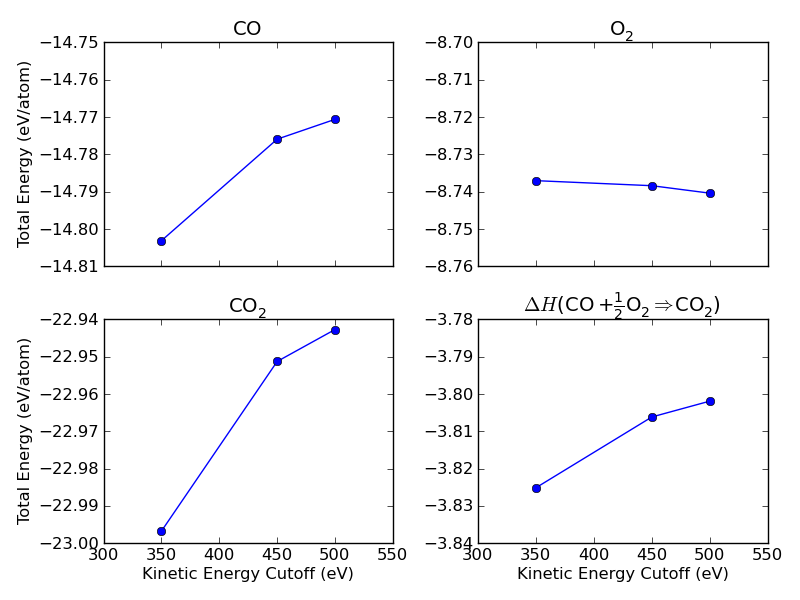
\includegraphics[width=0.7\textwidth]{./1b.png}
\caption{Convergence of CO, O$_{2}$, CO$_{2}$, and the reaction enthalpy of CO + 1/2O$_{2}$ $\rightarrow$ CO$_{2}$ with respect to plane wave cutoff energy}
\end{figure}

The total energy of the oxygen molecule converges the fastest. Note, all y-axis tick spacings are the same.
\section{Zero-point energy corrections}
\label{sec-2}
\subsection{Compute vibrational modes for CO, CO$_{2}$ and O$_{2}$}
\label{sec-2-1}

Compute the vibrational modes of each molecule in the CO oxidation reaction. Do this at 350 eV cutoff energy only. Prepare a table of the vibrational modes for molecule.


\begin{minted}[frame=lines,fontsize=\scriptsize,linenos]{python}
import os
import sys
from ase.calculators.vasp import Vasp
import ase.units
from jasp import *

# Since we wanted relaxed molecules for these calculations, we can take
# these geometries from the previous problem.

with jasp('prob1b/e350/CO') as calc:
    CO = calc.get_atoms()
with jasp('prob1b/e350/O2') as calc:
    O2 = calc.get_atoms()
with jasp('prob1b/e350/CO2') as calc:
    CO2 = calc.get_atoms()

# Now we're ready to perform the vibrational calculations
with jasp('prob2a/CO',
          xc='PBE', lreal=False,
          encut=350, prec='Accurate', ediff=1e-8,
          kpts=(1, 1, 1), ismear=0, sigma=0.05,
          ibrion=6, nsw=1, potim=0.015, nfree=2,
          atoms=CO) as calcCO:
    try:
        CO.get_potential_energy()
        energies, modes = calcCO.get_vibrational_modes()
        print 'Energies of CO\n======='
        for i, e in enumerate(energies):
            print '{0:02d}: {1} eV'.format(i, e)
    except:
        pass
with jasp('prob2a/O2',
          xc='PBE', lreal=False,
          encut=350, prec='Accurate', ediff=1e-8,
          kpts=(1, 1, 1), ismear=0, sigma=0.05,
          ibrion=6, nsw=1, potim=0.015, nfree=2,
          atoms=O2) as calcO2:
    try:
        O2.get_potential_energy()
        energies, modes = calcO2.get_vibrational_modes()
        print '\nEnergies of O2\n======='
        for i, e in enumerate(energies):
            print '{0:02d}: {1} eV'.format(i, e)
    except:
        pass
with jasp('prob2a/CO2',
          xc='PBE', lreal=False,
          encut=350, prec='Accurate', ediff=1e-8,
          kpts=(1, 1, 1), ismear=0, sigma=0.05,
          ibrion=6, nsw=1, potim=0.015, nfree=2,
          atoms=CO2) as calcCO2:
    try:
        CO2.get_potential_energy()
        energies, modes = calcCO2.get_vibrational_modes()
        print '\nEnergies of CO2\n======'
        for i, e in enumerate(energies):
            print '{0:02d}: {1} eV'.format(i, e)
    except:
        pass
\end{minted}


\begin{verbatim}
Energies of CO
=======
00: 0.261840727 eV
01: 0.003767323 eV
02: 0.003767323 eV
03: (3.0739e-05+0j) eV
04: (0.000943898+0j) eV
05: (0.000943898+0j) eV

Energies of O2
=======
00: 0.189490603 eV
01: 0.004093929 eV
02: 1e-09 eV
03: 0.0 eV
04: (1e-09+0j) eV
05: (0.006638148+0j) eV

Energies of CO2
======
00: 0.291924562 eV
01: 0.16318552 eV
02: 0.078492458 eV
03: 0.078492458 eV
04: 0.004836504 eV
05: 0.004836504 eV
06: (4.1677e-05+0j) eV
07: (5.9833e-05+0j) eV
08: (5.9833e-05+0j) eV
\end{verbatim}
\subsection{Compute the CO oxidation reaction energy with zero-point energy corrections.}
\label{sec-2-2}

Compare the reaction energy with and without the zero-point energy correction.


\begin{minted}[frame=lines,fontsize=\scriptsize,linenos]{python}
from jasp import *
import numpy as np
c = 3e10 # speed of light cm/s
h = 4.135667516e-15 # eV/s

# Get the vibrational energies from problem 2a. Get the total energies from 
# problem 1b at 350 eV.

with jasp('prob2a/CO') as calc:
    COfreq = calc.get_vibrational_frequencies()
with jasp('prob1b/e350/CO') as calc:
    atoms = calc.get_atoms()
    COe = atoms.get_potential_energy()
for f in COfreq:
    if not isinstance(f, float):
        continue
    nu = f*c
    COe += 0.5*h*nu
with jasp('prob2a/O2') as calc:
    O2freq = calc.get_vibrational_frequencies()
with jasp('prob1b/e350/O2') as calc:
    atoms = calc.get_atoms()
    O2e = atoms.get_potential_energy()
for f in O2freq:
    if not isinstance(f, float):
        continue
    nu = f*c
    O2e += 0.5*h*nu
with jasp('prob2a/CO2') as calc:
    CO2freq = calc.get_vibrational_frequencies()
with jasp('prob1b/e350/CO2') as calc:
    atoms = calc.get_atoms()
    CO2e = atoms.get_potential_energy()
for f in CO2freq:
    if not isinstance(f, float):
        continue
    nu = f*c
    CO2e += 0.5*h*nu
s = 'The reaction energy for CO oxidation with zero point contributions is {0:1.3f}'
print s.format(CO2e - COe - 0.5*O2e)
\end{minted}

\begin{verbatim}
 The reaction energy for CO oxidation with zero point contributions is -3.697
\end{verbatim}
\subsection{Compare your computed energy to a value from the literature.}
\label{sec-2-3}

Provide a reference for your literature value.

All values are taken from the NIST-JANAF Thermochemical Tables at kinetics.nist.gov/janaf.


\begin{minted}[frame=lines,fontsize=\scriptsize,linenos]{python}
# Values of heats of formation at 0 K in kJ/mol
Hf_CO = -113.805
Hf_CO2 = -393.151
Hf_O2 = 0 # Pure component is reference

Hf_rxn = -393.151 + 113.805
s = 'The experimental heat of reaction is {0:1.3f} eV/atom'
print s.format(Hf_rxn * 0.010364)
\end{minted}

\begin{verbatim}
 The experimental heat of reaction is -2.895 eV/atom
\end{verbatim}

Our computed heat of reaction is too exothermic. This means that either the products
(CO$_{2}$) are too stable, or the reactants (O$_{2}$ and CO) are unstable.
\section{Plot the electron density of the CO2 molecule.}
\label{sec-3}

Include the figure in your homework.

\begin{minted}[frame=lines,fontsize=\scriptsize,linenos]{python}
from jasp import *
from enthought.mayavi import mlab
from ase.data import vdw_radii
from ase.data.colors import cpk_colors
from ase import Atom, Atoms

# Lets first get the relaxed CO at 500 eV plane wave cutoff, center it,
# and recalculate the electron density in the centered cell

with jasp('prob1b/e500/CO') as calc:
    CO = calc.get_atoms()
    CO.center()
with jasp('prob3a/CO-centered',
          xc='PBE', lreal=False,
          encut=500, prec='Accurate',
          kpts=(1, 1, 1), ismear=1, sigma=0.05,
          atoms=CO) as calc:  
    CO.get_potential_energy()
    x, y, z, cd = calc.get_charge_density()

mlab.figure(bgcolor=(1, 1, 1))
# plot the atoms as spheres
for atom in CO:
    mlab.points3d(atom.x,
                  atom.y,
                  atom.z,
                  scale_factor=vdw_radii[atom.number]/5.,
                  resolution=20,
                  # a tuple is required for the color
                  color=tuple(cpk_colors[atom.number]),
                  scale_mode='none')

# draw the unit cell - there are 8 corners, and 12 connections
a1, a2, a3 = CO.get_cell()
origin = [0, 0, 0]
cell_matrix = [[origin,  a1],
               [origin,  a2],
               [origin,  a3],
               [a1,      a1 + a2],
               [a1,      a1 + a3],
               [a2,      a2 + a1],
               [a2,      a2 + a3],
               [a3,      a1 + a3],
               [a3,      a2 + a3],
               [a1 + a2, a1 + a2 + a3],
               [a2 + a3, a1 + a2 + a3],
               [a1 + a3, a1 + a3 + a2]]

for p1, p2 in cell_matrix:
    mlab.plot3d([p1[0], p2[0]], # x-positions
                [p1[1], p2[1]], # y-positions
                [p1[2], p2[2]], # z-positions
                tube_radius=0.02)

# Now plot the charge density
mlab.contour3d(x, y, z, cd, transparent=True)

# this view was empirically found by iteration
mlab.view(azimuth=-90, elevation=90, distance='auto')

mlab.savefig('co-density.png')
\end{minted}


\begin{figure}[H]
\centering
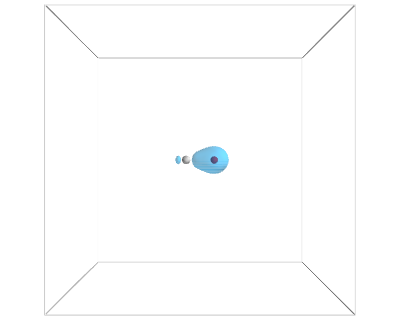
\includegraphics[width=0.7\textwidth]{./co-density.png}
\caption{Charge density of CO}
\end{figure}

\end{document}
